\documentclass{article}
\usepackage[T1]{fontenc}
\usepackage{lmodern}
\usepackage{graphicx}
\usepackage{amsmath,amssymb}
\usepackage[a4paper,margin=2cm]{geometry}
\usepackage[absolute,overlay]{textpos}
\setlength{\TPHorizModule}{1mm}
\setlength{\TPVertModule}{1mm}
\usepackage[indonesian]{babel}
\usepackage{hyperref}
\setlength{\emergencystretch}{2em}
% unit: Halaman 13

\begin{document}

% === Halaman 13 (python/native) ===

• Penggunaan tablet wax 

 Orang-orang Yunani kuno menulis pesan rahasia di atas kayu yang kemudian 

ditutup dengan lilin (wax).


 Di dalam bukunya, Heradatus menceritakan Demaratus mengirim peringatan 

tentang serangan yang akan datang ke Yunani dengan menulis langsung pada 

tablet kayu yang kemudian dilapisi lilin dari lebah.  

13

% deskripsi: gambar native xref 100
\noindent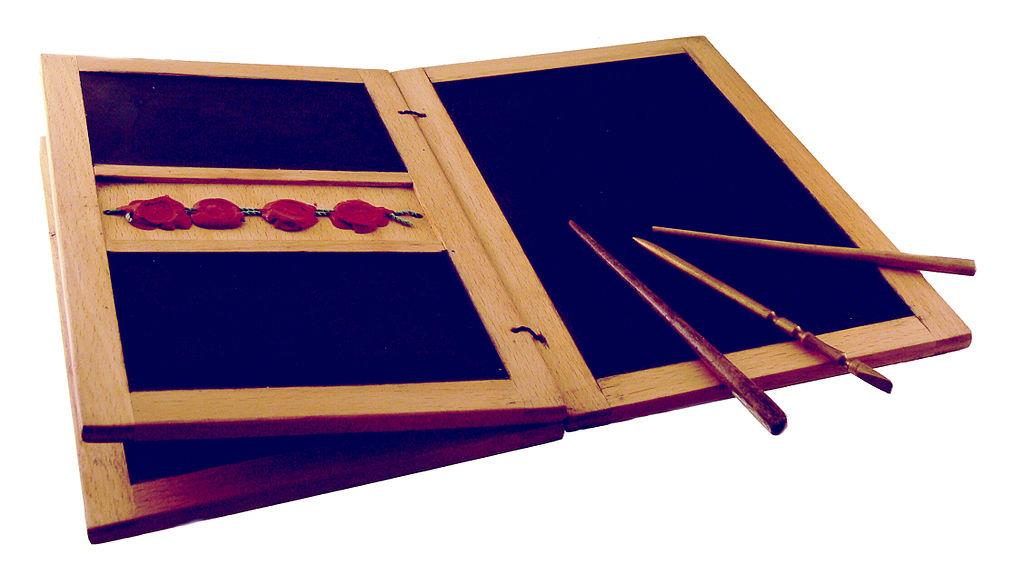
\includegraphics[width=0.85\textwidth]{../../images/python/page_013_img_01.jpeg}

\end{document}
